%==========================================================
% CHAPTER: Lygtys ir nelygybės su moduliais (A kursas)
%==========================================================
\chapter{Lygtys ir nelygybės su moduliais (A kursas)}

\section{Absoliučiosios vertės sąvoka}

\subsection{Apibrėžimas ir geometrinė prasmė}

\begin{definition}
Realaus skaičiaus $x$ \textbf{absoliučioji vertė} (arba \textbf{modulis}) žymima $|x|$ ir apibrėžiama:
\[
|x| =
\begin{cases}
x, & \text{jei } x \geq 0, \\
-x, & \text{jei } x < 0.
\end{cases}
\]
\end{definition}

\begin{remark}
Absoliučioji vertė visada yra neneigiama: $|x| \geq 0$ kiekvienam $x \in \mathbb{R}$.
\end{remark}

\subsubsection*{Geometrinė prasmė}

Skaičių tiesėje skaičiaus $x$ absoliučioji vertė $|x|$ reiškia \textbf{atstumą nuo taško $x$ iki koordinačių pradžios taško $0$}.

\begin{center}
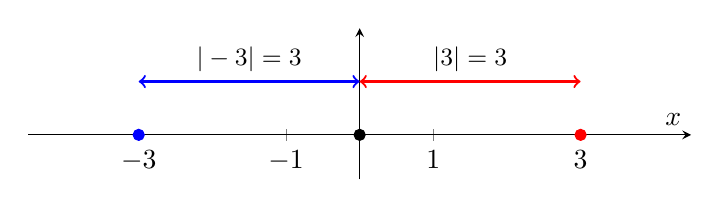
\begin{tikzpicture}
\begin{axis}[
    axis lines=center,
    xlabel={$x$},
    xmin=-4.5, xmax=4.5,
    ymin=-0.5, ymax=1.2,
    ytick=\empty,
    xtick={-3,-1,0,1,3},
    xticklabels={$-3$,$-1$,$0$,$1$,$3$},
    width=10cm, height=3.5cm,
    clip=false
]
\addplot[thick, blue, <->] coordinates {(-3,0.6)(0,0.6)};
\addplot[thick, red, <->] coordinates {(0,0.6)(3,0.6)};
\node[above] at (axis cs:-1.5,0.6) {\small $|-3|=3$};
\node[above] at (axis cs:1.5,0.6) {\small $|3|=3$};
\addplot[mark=*,blue] coordinates {(-3,0)};
\addplot[mark=*,red] coordinates {(3,0)};
\addplot[mark=*,black] coordinates {(0,0)};
\end{axis}
\end{tikzpicture}
\end{center}

Plačiau: $|a - b|$ reiškia \textbf{atstumą tarp taškų $a$ ir $b$} skaičių tiesėje.

\begin{example}
Apskaičiuokime kelių skaičių absoliučiąsias vertes:
\begin{itemize}
    \item $|5| = 5$
    \item $|-7| = 7$
    \item $|0| = 0$
    \item $|-\tfrac{3}{4}| = \tfrac{3}{4}$
    \item $|\sqrt{2} - 2| = 2 - \sqrt{2}$, nes $\sqrt{2} < 2$, todėl $\sqrt{2}-2 < 0$.
\end{itemize}
\end{example}

\begin{example}
Išspręskime nelygybes geometriniu būdu:
\begin{enumerate}[label=\alph*)]
    \item $|x| < 3$ reiškia, kad $x$ nutolęs nuo $0$ mažiau nei $3$, t.~y. $-3 < x < 3$.
    \item $|x - 1| \leq 2$ reiškia, kad $x$ nutolęs nuo taško $1$ ne daugiau kaip $2$, t.~y. $-1 \leq x \leq 3$.
\end{enumerate}
\end{example}

\subsection{Absoliučiosios vertės savybės}

Toliau pateikiamos pagrindinės absoliučiosios vertės savybės, kurios naudojamos sprendžiant lygtis ir nelygybes.

\begin{theorem}[Pagrindinės savybės]
\label{thm:abs_savybes}
Tebūna $a, b \in \mathbb{R}$. Tada:
\begin{enumerate}[label=\arabic*.]
    \item $|a| \geq 0$ ir $|a| = 0 \iff a = 0$ \hfill \emph{(neneigiamumas)}
    \item $|-a| = |a|$ \hfill \emph{(lyginumas)}
    \item $|a|^2 = a^2$ \hfill \emph{(kvadratas)}
    \item $|a \cdot b| = |a| \cdot |b|$ \hfill \emph{(sandaugos savybė)}
    \item $\left|\dfrac{a}{b}\right| = \dfrac{|a|}{|b|}$, kai $b \neq 0$ \hfill \emph{(dalmens savybė)}
    \item $|a + b| \leq |a| + |b|$ \hfill \emph{(trikampio nelygybė)}
    \item $\bigl||a| - |b|\bigr| \leq |a - b|$ \hfill \emph{(atvirkštinė trikampio nelygybė)}
\end{enumerate}
\end{theorem}

\begin{proof}[Sandaugos savybės įrodymas]
Pasinaudojame savybe $|x|^2 = x^2$:
\[
|a \cdot b|^2 = (ab)^2 = a^2 b^2 = |a|^2 \cdot |b|^2 = \bigl(|a| \cdot |b|\bigr)^2.
\]
Kadangi $|ab| \geq 0$ ir $|a|\cdot|b| \geq 0$, tai $|ab| = |a| \cdot |b|$.
\end{proof}

\begin{tcolorbox}[title={Trikampio nelygybė}, colback=blue!5!white, colframe=blue!60!black]
Svarbi trikampio nelygybė:
\[
|a + b| \leq |a| + |b|, \quad \forall\, a, b \in \mathbb{R}.
\]
Lygybė galioja tada ir tik tada, kai $a$ ir $b$ yra vienodų ženklų (arba bent vienas jų lygus nuliui), t.~y. $ab \geq 0$.
\end{tcolorbox}

\subsubsection*{Absoliučiosios vertės ir lygčių / nelygybių sąryšis}

\begin{theorem}
Tebūna $c > 0$. Tada:
\begin{align*}
|x| = c &\iff x = c \;\text{ arba }\; x = -c, \\
|x| < c &\iff -c < x < c, \\
|x| > c &\iff x > c \;\text{ arba }\; x < -c, \\
|x| \leq c &\iff -c \leq x \leq c, \\
|x| \geq c &\iff x \geq c \;\text{ arba }\; x \leq -c.
\end{align*}
\end{theorem}

\begin{example}
Išspręskite lygtis ir nelygybes:
\begin{enumerate}[label=\alph*)]
    \item $|2x - 3| = 5$\\
    Sprendimas: $2x - 3 = 5$ arba $2x - 3 = -5$, todėl $x = 4$ arba $x = -1$.

    \item $|3x + 1| < 7$\\
    Sprendimas: $-7 < 3x + 1 < 7 \Rightarrow -8 < 3x < 6 \Rightarrow x \in \left(-\tfrac{8}{3};\, 2\right)$.

    \item $|x - 2| \geq 3$\\
    Sprendimas: $x - 2 \geq 3$ arba $x - 2 \leq -3$, todėl $x \geq 5$ arba $x \leq -1$, t.~y. $x \in (-\infty;\,-1\,] \cup [\,5;\,+\infty)$.
\end{enumerate}
\end{example}

\begin{exercise}
Išspręskite lygtis:
\begin{enumerate}[label=\arabic*.]
    \item $|x + 4| = 6$
    \item $|2x - 1| = |x + 3|$
    \item $|x^2 - 4| = 0$
    \item $\left|\dfrac{x-1}{x+2}\right| = 1$, kai $x \neq -2$
\end{enumerate}
\end{exercise}

\begin{exercise}
Išspręskite nelygybes:
\begin{enumerate}[label=\arabic*.]
    \item $|5x - 2| \leq 8$
    \item $|x + 3| > 4$
    \item $|2x + 1| - 3 < 0$
    \item $|x - 1| + |x + 1| \geq 4$
\end{enumerate}
\end{exercise}

\begin{remark}
Lygčiai $|f(x)| = |g(x)|$ spręsti naudojame ekvivalentiją:
\[
|f(x)| = |g(x)| \iff f(x) = g(x) \;\text{ arba }\; f(x) = -g(x).
\]
\end{remark}

\section{Lygtys su moduliais}

Lygtys su moduliais yra lygtys, kuriose nežinomasis yra po absoliučiosios vertės (modulio) ženklu. Prieš sprendžiant tokias lygtis, būtina prisiminti modulio apibrėžtį.

\begin{definition}
Skaičiaus $a$ \textbf{modulis} (absoliučioji vertė) apibrėžiamas taip:
\[
|a| = \begin{cases} a, & \text{jei } a \geq 0, \\ -a, & \text{jei } a < 0. \end{cases}
\]
\end{definition}

\begin{tcolorbox}[colback=blue!5!white, colframe=blue!60!black, title=Pagrindinės modulio savybės]
\begin{itemize}
    \item $|a| \geq 0$ visiems $a \in \mathbb{R}$;
    \item $|a| = 0 \iff a = 0$;
    \item $|-a| = |a|$;
    \item $|a \cdot b| = |a| \cdot |b|$;
    \item $\left|\dfrac{a}{b}\right| = \dfrac{|a|}{|b|}$, $b \neq 0$;
    \item $|a + b| \leq |a| + |b|$ \quad (trikampio nelygybė).
\end{itemize}
\end{tcolorbox}

\begin{remark}
Geometrine prasme $|a|$ reiškia atstumo nuo taško $a$ iki nulio skaičių tiesėje. Analogiškai $|a - b|$ yra atstumas tarp taškų $a$ ir $b$ skaičių tiesėje.
\end{remark}

% ----------------------------------------------------------------
\subsection{Paprasčiausios lygtys \texorpdfstring{$|f(x)| = a$}{|f(x)| = a}}

Šio tipo lygtyse po modulio ženklo stovi funkcija $f(x)$, o dešinėje pusėje -- skaičius $a$.

\begin{theorem}
Tegu $a \in \mathbb{R}$. Tada:
\begin{itemize}
    \item Jei $a < 0$, lygtis $|f(x)| = a$ \textbf{sprendimų neturi}, nes modulis visada yra neneigiamas.
    \item Jei $a = 0$, lygtis $|f(x)| = 0$ ekvivalenti lygčiai $f(x) = 0$.
    \item Jei $a > 0$, lygtis $|f(x)| = a$ ekvivalenti dviem lygtims:
    \[
    f(x) = a \quad \text{arba} \quad f(x) = -a.
    \]
\end{itemize}
\end{theorem}

\begin{tcolorbox}[colback=green!5!white, colframe=green!50!black, title={Sprendimo algoritmas: $|f(x)| = a$}]
\begin{enumerate}
    \item Patikrinti, ar $a \geq 0$. Jei $a < 0$ -- sprendimų nėra.
    \item Jei $a \geq 0$, sudaryti dvi lygtis: $f(x) = a$ ir $f(x) = -a$.
    \item Išspręsti abi lygtis.
    \item Atsakymui sujungti abiejų lygčių sprendinius.
\end{enumerate}
\end{tcolorbox}

\begin{example}
Išspręsti lygtį $|x - 3| = 5$.

\textbf{Sprendimas.}

Kadangi $a = 5 > 0$, lygtis ekvivalenti dviem lygtims:
\[
x - 3 = 5 \quad \text{arba} \quad x - 3 = -5.
\]
Iš pirmosios: $x = 8$.\\
Iš antrosios: $x = -2$.

\textbf{Atsakymas:} $x = 8$ arba $x = -2$.
\end{example}

\begin{example}
Išspręsti lygtį $|2x + 1| = 7$.

\textbf{Sprendimas.}

$2x + 1 = 7$ arba $2x + 1 = -7$.

Iš pirmosios: $2x = 6$, taigi $x = 3$.\\
Iš antrosios: $2x = -8$, taigi $x = -4$.

\textbf{Atsakymas:} $x = 3$ arba $x = -4$.
\end{example}

\begin{example}
Išspręsti lygtį $3|x + 2| - 1 = 8$.

\textbf{Sprendimas.}

Pirmiausia išskiriame modulį:
\[
3|x + 2| = 9 \implies |x + 2| = 3.
\]
Tada:
\[
x + 2 = 3 \quad \text{arba} \quad x + 2 = -3.
\]
Iš pirmosios: $x = 1$.\\
Iš antrosios: $x = -5$.

\textbf{Atsakymas:} $x = 1$ arba $x = -5$.
\end{example}

\begin{example}
Išspręsti lygtį $|x^2 - 4| = 0$.

\textbf{Sprendimas.}

Kadangi $a = 0$, lygtis ekvivalenti:
\[
x^2 - 4 = 0 \implies x^2 = 4 \implies x = \pm 2.
\]

\textbf{Atsakymas:} $x = 2$ arba $x = -2$.
\end{example}

\begin{example}
Išspręsti lygtį $|x^2 - 5x + 6| = 0$.

\textbf{Sprendimas.}

\[
x^2 - 5x + 6 = 0.
\]
Diskriminantas: $D = 25 - 24 = 1$.
\[
x_1 = \frac{5 - 1}{2} = 2, \quad x_2 = \frac{5 + 1}{2} = 3.
\]

\textbf{Atsakymas:} $x = 2$ arba $x = 3$.
\end{example}

\begin{remark}
Kai $a < 0$, lygtis $|f(x)| = a$ neturi sprendimų, nes $|f(x)| \geq 0$ visiems $x$. Pavyzdžiui, lygtis $|x + 1| = -3$ neturi sprendimų.
\end{remark}

\begin{exercise}
Išspręsti lygtis:
\begin{enumerate}[label=\alph*)]
    \item $|x + 5| = 3$
    \item $|3x - 2| = 7$
    \item $2|x - 1| + 4 = 10$
    \item $|x^2 - 9| = 0$
    \item $|5 - 2x| = -1$
\end{enumerate}
\end{exercise}

% ----------------------------------------------------------------
\subsection{Lygtys \texorpdfstring{$|f(x)| = g(x)$}{|f(x)| = g(x)}}

Šio tipo lygtyse modulio ženklo dešinėje pusėje stovi ne skaičius, o funkcija $g(x)$. Tai reikalauja papildomo atidumo, nes sprendiniai turi tenkinti sąlygą $g(x) \geq 0$.

\begin{theorem}
Lygtis $|f(x)| = g(x)$ ekvivalenti sistemai:
\[
\left[
\begin{array}{l}
\begin{cases} f(x) = g(x), \\ g(x) \geq 0, \end{cases} \\[8pt]
\begin{cases} f(x) = -g(x), \\ g(x) \geq 0. \end{cases}
\end{array}
\right.
\]
arba, supaprastintai, dviem lygtims su patikrinimu:
\[
f(x) = g(x) \quad \text{arba} \quad f(x) = -g(x),
\]
kur kiekvieną gautą sprendinį $x_0$ reikia \textbf{patikrinti}, ar $g(x_0) \geq 0$.
\end{theorem}

\begin{tcolorbox}[colback=green!5!white, colframe=green!50!black, title={Sprendimo algoritmas: $|f(x)| = g(x)$}]
\begin{enumerate}
    \item Sudaryti dvi lygtis: $f(x) = g(x)$ ir $f(x) = -g(x)$.
    \item Išspręsti abi lygtis.
    \item \textbf{Patikrinti} kiekvieną sprendinį: įstatyti į $g(x)$ ir įsitikinti, kad $g(x) \geq 0$. Sprendiniai, kurių $g(x) < 0$, atmetami.
\end{enumerate}
\end{tcolorbox}

\begin{example}
Išspręsti lygtį $|x - 2| = x + 4$.

\textbf{Sprendimas.}

Sudarome dvi lygtis:
\[
x - 2 = x + 4 \quad \text{arba} \quad x - 2 = -(x + 4).
\]

\textit{1 lygtis:} $x - 2 = x + 4 \implies -2 = 4$ -- prieštaravimas, sprendinių nėra.

\textit{2 lygtis:}
\[
x - 2 = -x - 4 \implies 2x = -2 \implies x = -1.
\]

\textit{Patikrinimas:} $g(-1) = (-1) + 4 = 3 \geq 0$ \checkmark

\textbf{Atsakymas:} $x = -1$.
\end{example}

\begin{example}
Išspręsti lygtį $|2x - 3| = x - 1$.

\textbf{Sprendimas.}

\textit{1 lygtis:}
\[
2x - 3 = x - 1 \implies x = 2.
\]
Patikrinimas: $g(2) = 2 - 1 = 1 \geq 0$ \checkmark

\textit{2 lygtis:}
\[
2x - 3 = -(x - 1) = -x + 1 \implies 3x = 4 \implies x = \frac{4}{3}.
\]
Patikrinimas: $g\!\left(\tfrac{4}{3}\right) = \tfrac{4}{3} - 1 = \tfrac{1}{3} \geq 0$ \checkmark

\textbf{Atsakymas:} $x = 2$ arba $x = \dfrac{4}{3}$.
\end{example}

\begin{example}
Išspręsti lygtį $|x + 3| = 2x - 5$.

\textbf{Sprendimas.}

\textit{1 lygtis:}
\[
x + 3 = 2x - 5 \implies -x = -8 \implies x = 8.
\]
Patikrinimas: $g(8) = 16 - 5 = 11 \geq 0$ \checkmark

\textit{2 lygtis:}
\[
x + 3 = -(2x - 5) = -2x + 5 \implies 3x = 2 \implies x = \frac{2}{3}.
\]
Patikrinimas: $g\!\left(\tfrac{2}{3}\right) = \tfrac{4}{3} - 5 = -\tfrac{11}{3} < 0$ ✗ -- atmetamas.

\textbf{Atsakymas:} $x = 8$.
\end{example}

\begin{remark}
Praleidus patikrinimo žingsnį, galima gauti klaidingus sprendinius (vadinamus \textit{pašaliniais}). Tai yra dažna klaida VBE, todėl patikrinimas yra \textbf{privalomas}.
\end{remark}

\begin{exercise}
Išspręsti lygtis:
\begin{enumerate}[label=\alph*)]
    \item $|x - 1| = 2x + 3$
    \item $|3x + 2| = x + 6$
    \item $|x^2 - 4| = x + 2$
    \item $|2x - 5| = x - 1$
\end{enumerate}
\end{exercise}

% ----------------------------------------------------------------
\subsection{Lygtys su keliais moduliais}

Sudėtingesnės lygtys gali turėti kelis modulius. Tokias lygtis sprendžiame dviem pagrindiniais metodais: \textbf{apibrėžties taikymo} (intervalų) metodu arba \textbf{kvadratu kėlimo} metodu.

\subsubsection{Intervalų metodas}

\begin{tcolorbox}[colback=green!5!white, colframe=green!50!black, title=Intervalų metodo algoritmas]
\begin{enumerate}
    \item Rasti visus \textbf{kritinius taškus} -- kintamojo reikšmes, kuriose kiekvienas modulio viduje esantis reiškinys lygi nuliui.
    \item Kritiniais taškais padalyti skaičių tiesę į \textbf{intervalus}.
    \item Kiekviename intervale nustatyti kiekvieno modulio ženklą ir \textbf{atsisakyti modulio ženklo} pagal apibrėžtį.
    \item Kiekviename intervale išspręsti gautą lygtį (be modulių).
    \item Patikrinti, ar sprendiniai priklauso atitinkamiems intervalams; neatitinkantys -- atmetami.
    \item Sujungti visų intervalų sprendinius.
\end{enumerate}
\end{tcolorbox}

\begin{example}
Išspręsti lygtį $|x - 1| + |x + 3| = 8$.

\textbf{Sprendimas.}

Kritiniai taškai: $x = 1$ ir $x = -3$.

Skaičių tiesė dalijama į tris intervalus:

\medskip
\begin{center}
\begin{tikzpicture}
\draw[->] (-6,0) -- (4,0) node[right] {$x$};
\foreach \x/\l in {-3/$-3$, 1/$1$}
    \draw (\x,0.1)--(\x,-0.1) node[below] {\l};
\node at (-4.5,0.4) {$x < -3$};
\node at (-1,0.4)   {$-3 \leq x < 1$};
\node at (2.5,0.4)  {$x \geq 1$};
\end{tikzpicture}
\end{center}

\medskip
\textit{1 intervalas: $x < -3$}

Abu reiškiniai neigiami:
\[
-(x-1) + (-(x+3)) = 8 \implies -x+1-x-3 = 8 \implies -2x = 10 \implies x = -5.
\]
Tikrinimas: $-5 < -3$ \checkmark

\textit{2 intervalas: $-3 \leq x < 1$}

$x - 1 < 0$, $x + 3 \geq 0$:
\[
-(x-1) + (x+3) = 8 \implies -x+1+x+3 = 8 \implies 4 = 8.
\]
Prieštaravimas -- intervale sprendinių nėra.

\textit{3 intervalas: $x \geq 1$}

Abu reiškiniai neneigiami:
\[
(x-1) + (x+3) = 8 \implies 2x + 2 = 8 \implies x = 3.
\]
Tikrinimas: $3 \geq 1$ \checkmark

\textbf{Atsakymas:} $x = -5$ arba $x = 3$.
\end{example}

\begin{example}
Išspręsti lygtį $|x + 2| - |x - 3| = 1$.

\textbf{Sprendimas.}

Kritiniai taškai: $x = -2$ ir $x = 3$.

\textit{1 intervalas: $x < -2$}
\[
-(x+2) - (-(x-3)) = 1 \implies -x-2+x-3 = 1 \implies -5 = 1.
\]
Prieštaravimas.

\textit{2 intervalas: $-2 \leq x < 3$}
\[
(x+2) - (-(x-3)) = 1 \implies x+2+x-3 = 1 \implies 2x - 1 = 1 \implies x = 1.
\]
Tikrinimas: $-2 \leq 1 < 3$ \checkmark

\textit{3 intervalas: $x \geq 3$}
\[
(x+2) - (x-3) = 1 \implies 5 = 1.
\]
Prieštaravimas.

\textbf{Atsakymas:} $x = 1$.
\end{example}

\subsubsection{Kvadratu kėlimo metodas}

Jei lygtis yra pavidalo $|f(x)| = |g(x)|$, naudingiau taikyti \textbf{kvadratu kėlimo metodą}.

\begin{theorem}
Lygtis $|f(x)| = |g(x)|$ ekvivalenti lygčiai:
\[
[f(x)]^2 = [g(x)]^2,
\]
nes $|a| = |b| \iff a^2 = b^2$.

Ši lygtis savo ruožtu ekvivalenti:
\[
f(x) = g(x) \quad \text{arba} \quad f(x) = -g(x).
\]
\end{theorem}

\begin{example}
Išspręsti lygtį $|2x - 1| = |x + 3|$.

\textbf{Sprendimas.}

Naudojame ekvivalentiškumą:
\[
2x - 1 = x + 3 \quad \text{arba} \quad 2x - 1 = -(x + 3).
\]

\textit{1 lygtis:} $2x - 1 = x + 3 \implies x = 4$.

\textit{2 lygtis:} $2x - 1 = -x - 3 \implies 3x = -2 \implies x = -\dfrac{2}{3}$.

\textbf{Atsakymas:} $x = 4$ arba $x = -\dfrac{2}{3}$.
\end{example}

\begin{example}
Išspręsti lygtį $|x^2 - 1| = |x - 1|$.

\textbf{Sprendimas.}

\textit{1 lygtis:}
\[
x^2 - 1 = x - 1 \implies x^2 - x = 0 \implies x(x-1) = 0 \implies x = 0 \text{ arba } x = 1.
\]

\textit{2 lygtis:}
\[
x^2 - 1 = -(x-1) = -x + 1 \implies x^2 + x - 2 = 0 \implies (x+2)(x-1) = 0 \implies x = -2 \text{ arba } x = 1.
\]

Sujungiame: $x \in \{-2,\; 0,\; 1\}$.

\textbf{Atsakymas:} $x = -2$, $x = 0$ arba $x = 1$.
\end{example}

\begin{remark}
Lygtims su daugiau nei dviem moduliais taikomas tas pats intervalų metodas -- tik kritinių taškų gali būti daugiau, todėl intervalų bus daugiau.
\end{remark}

\begin{example}
Išspręsti lygtį $|x| + |x - 1| + |x + 1| = 3$.

\textbf{Sprendimas.}

Kritiniai taškai: $x = -1$, $x = 0$, $x = 1$. Keturi intervalai:

\medskip
\textit{1 intervalas: $x < -1$}
\[
(-x) + (-(x-1)) + (-(x+1)) = 3 \implies -3x = 3 \implies x = -1.
\]
Bet $-1 \not< -1$, atmetama.

\textit{2 intervalas: $-1 \leq x < 0$}
\[
(-x) + (-(x-1)) + (x+1) = 3 \implies -x + 2 = 3 \implies x = -1.
\]
Tikrinimas: $-1 \leq -1 < 0$ \checkmark \quad $x = -1$.

\textit{3 intervalas: $0 \leq x < 1$}
\[
x + (-(x-1)) + (x+1) = 3 \implies x + 2 = 3 \implies x = 1.
\]
Bet $1 \not< 1$, atmetama.

\textit{4 intervalas: $x \geq 1$}
\[
x + (x-1) + (x+1) = 3 \implies 3x = 3 \implies x = 1.
\]
Tikrinimas: $1 \geq 1$ \checkmark

\textbf{Atsakymas:} $x = -1$ arba $x = 1$.
\end{example}

\begin{exercise}
Išspręsti lygtis:
\begin{enumerate}[label=\alph*)]
    \item $|x + 1| + |x - 2| = 5$
    \item $|x - 3| - |x + 1| = 2$
    \item $|2x - 1| = |x + 4|$
    \item $|x| + |x + 2| + |x - 2| = 6$
    \item $|x^2 - 4| = |2x - 4|$
\end{enumerate}
\end{exercise}

\begin{tcolorbox}[colback=yellow!10!white, colframe=orange!70!black, title=VBE patarimai: lygtys su moduliais]
\begin{itemize}
    \item Visada \textbf{patikrinkite} gautus sprendinius originalioje lygtyje -- ypač kai dešinėje yra $g(x)$.
    \item Tipo $|f(x)| = a < 0$ lygtys neturi sprendimų -- nerašykite jokių atsakymų.
    \item Intervalų metode po sprendimo patikrinkite, ar sprendinys iš tikrųjų priklauso nagrinėtam intervalui.
    \item Lygtims $|f(x)| = |g(x)|$ dažnai greičiau ir patikimiau yra kvadratu kėlimo metodas.
    \item Naudokite skaičiuotuvą patikrinimui, bet pilną sprendimą rašykite \textbf{algebriškai}.
\end{itemize}
\end{tcolorbox}

\section{Nelygybės su moduliais}

Modulis yra skaičiaus atstumas nuo nulio skaičių tiesėje. Formaliai:

\begin{definition}
Skaičiaus $x$ \textbf{modulis} (arba absoliutioji reikšmė) apibrėžiamas taip:
\[
|x| =
\begin{cases}
x, & \text{jei } x \geq 0, \\
-x, & \text{jei } x < 0.
\end{cases}
\]
\end{definition}

\begin{remark}
Modulis visada yra neneigiamas: $|x| \geq 0$ visiems $x \in \mathbb{R}$.
Geometriškai $|x - a|$ reiškia atstumą tarp taškų $x$ ir $a$ skaičių tiesėje.
\end{remark}

% -------------------------------------------------------
\subsection{Nelygybės \texorpdfstring{$|f(x)| < a$}{|f(x)| < a} ir \texorpdfstring{$|f(x)| > a$}{|f(x)| > a}}

Kai dešinėje nelygybės pusėje yra teigiamas skaičius $a > 0$, taikomos šios taisyklės:

\begin{tcolorbox}[title=Pagrindinės taisyklės ($a > 0$), colback=blue!5, colframe=blue!60]
\begin{enumerate}[label=\textbf{\arabic*.}]
  \item $|f(x)| < a \iff -a < f(x) < a$
  \item $|f(x)| \leq a \iff -a \leq f(x) \leq a$
  \item $|f(x)| > a \iff f(x) < -a \;\text{ arba }\; f(x) > a$
  \item $|f(x)| \geq a \iff f(x) \leq -a \;\text{ arba }\; f(x) \geq a$
\end{enumerate}
\end{tcolorbox}

\begin{remark}
Geometrinė prasmė: $|f(x)| < a$ reiškia, kad $f(x)$ reikšmė patenka į intervalą $(-a,\, a)$, t.\,y. nutolsta nuo nulio mažiau nei $a$. Tuo tarpu $|f(x)| > a$ reiškia, kad $f(x)$ nutolsta nuo nulio daugiau nei $a$.
\end{remark}

\begin{tcolorbox}[title=Ypatingi atvejai, colback=yellow!10, colframe=orange!70]
\begin{itemize}
  \item Jei $a \leq 0$: nelygybė $|f(x)| < a$ \textbf{neturi sprendinių} (modulis negali būti neigiamas).
  \item Jei $a \leq 0$: nelygybė $|f(x)| > a$ \textbf{teisinga visiems} $x$ (modulis visada $\geq 0 > a$).
  \item $|f(x)| \leq 0 \iff f(x) = 0$.
  \item $|f(x)| \geq 0$ teisinga visiems $x \in \mathbb{R}$.
\end{itemize}
\end{tcolorbox}

\subsubsection*{Sprendimo algoritmas (kai $a > 0$)}

\begin{enumerate}
  \item Nustatyti nelygybės tipą: $|f(x)| < a$ arba $|f(x)| > a$.
  \item Taikyti atitinkamą taisyklę ir gauti ekvivalenčią nelygybę be modulio ženklo.
  \item Išspręsti gautą nelygybę ar nelygybių sistemą.
  \item Parašyti atsakymą intervalo arba nelygybės forma.
\end{enumerate}

\begin{example}
Išspręskite nelygybę $|2x - 3| < 5$.

\textbf{Sprendimas.}

Taikome taisyklę $|f(x)| < a \iff -a < f(x) < a$:
\[
-5 < 2x - 3 < 5.
\]
Pridedame $3$ prie visų dalių:
\[
-2 < 2x < 8.
\]
Dalijame iš $2$:
\[
-1 < x < 4.
\]

\textbf{Atsakymas:} $x \in (-1;\, 4)$.
\end{example}

\begin{example}
Išspręskite nelygybę $|3x + 1| \geq 7$.

\textbf{Sprendimas.}

Taikome taisyklę $|f(x)| \geq a \iff f(x) \leq -a \text{ arba } f(x) \geq a$:
\[
3x + 1 \leq -7 \quad \text{arba} \quad 3x + 1 \geq 7.
\]
Pirmoji nelygybė:
\[
3x \leq -8 \implies x \leq -\frac{8}{3}.
\]
Antroji nelygybė:
\[
3x \geq 6 \implies x \geq 2.
\]

\textbf{Atsakymas:} $x \in \left(-\infty;\, -\dfrac{8}{3}\right] \cup [2;\, +\infty)$.
\end{example}

\begin{example}
Išspręskite nelygybę $\left|\dfrac{x-1}{2}\right| < -3$.

\textbf{Sprendimas.}

Kadangi $a = -3 < 0$, o modulis visada yra neneigiamas ($|\cdot| \geq 0 > -3$), ši nelygybė \textbf{neturi sprendinių}.

\textbf{Atsakymas:} $\varnothing$.
\end{example}

\begin{example}
Nubraižykite skaičių tiesėje nelygybės $|x - 2| < 3$ sprendinių aibę.

\textbf{Sprendimas.}

\[
-3 < x - 2 < 3 \implies -1 < x < 5.
\]

\begin{center}
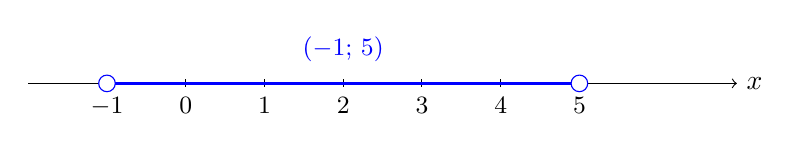
\begin{tikzpicture}
  \draw[->] (-2,0) -- (7,0) node[right] {$x$};
  \foreach \x in {-1,0,1,2,3,4,5}
    \draw (\x,0.05) -- (\x,-0.05) node[below] {\small$\x$};
  \draw[very thick, blue] (-1,0) -- (5,0);
  \draw[blue, fill=white] (-1,0) circle (3pt);
  \draw[blue, fill=white] (5,0) circle (3pt);
  \node[blue, above] at (2, 0.15) {\small $(-1;\,5)$};
\end{tikzpicture}
\end{center}

\textbf{Atsakymas:} $x \in (-1;\, 5)$.
\end{example}

% -------------------------------------------------------
\subsection{Sudėtingesnės nelygybės su moduliais}

Kai modulio viduje yra sudėtingesnis reiškinys arba kai nelygybėje figūruoja keli moduliai, naudojami šie metodai:

\begin{enumerate}[label=\textbf{\Roman*.}]
  \item \textbf{Modulio apibrėžimo taikymas} (atvejų nagrinėjimas)
  \item \textbf{Intervalų metodas}
  \item \textbf{Kvadratavimas} (tik kai abi pusės neneigiamos)
\end{enumerate}

% --- I metodas ---
\subsubsection*{I metodas: Atvejų nagrinėjimas}

Išreiškiame modulį pagal apibrėžimą ir nagrinėjame du atvejus.

\begin{example}
Išspręskite nelygybę $|x^2 - 4| > x + 2$.

\textbf{Sprendimas.}

Randame nulinį modulio tašką: $x^2 - 4 = 0 \Rightarrow x = \pm 2$.

\textbf{1 atvejis:} $x \leq -2$ arba $x \geq 2$. Tada $|x^2 - 4| = x^2 - 4$.
\[
x^2 - 4 > x + 2 \implies x^2 - x - 6 > 0 \implies (x-3)(x+2) > 0.
\]
Sprendiniai: $x < -2$ arba $x > 3$.
Sukirsdami su šio atvejo sąlyga: $x < -2$ arba $x > 3$.

\textbf{2 atvejis:} $-2 < x < 2$. Tada $|x^2 - 4| = -(x^2 - 4) = 4 - x^2$.
\[
4 - x^2 > x + 2 \implies x^2 + x - 2 < 0 \implies (x+2)(x-1) < 0.
\]
Sprendiniai: $-2 < x < 1$.
Sukirsdami su šio atvejo sąlyga: $-2 < x < 1$.

\textbf{Atsakymas:} $x \in (-\infty;\, -2) \cup (-2;\, 1) \cup (3;\, +\infty)$,
t.\,y. $x \in (-\infty;\, 1) \cup (3;\, +\infty)$ (nes $x = -2$ netenkina pradinės nelygybės).
\end{example}

% --- II metodas ---
\subsubsection*{II metodas: Intervalų metodas}

Šis metodas ypač patogus, kai nelygybėje yra \textbf{keli moduliai}.

\begin{tcolorbox}[title=Intervalų metodo žingsniai, colback=green!5, colframe=green!60]
\begin{enumerate}
  \item Rasti visus \textbf{nulinius taškus} – reikšmes, kurioms modulių vidiniai reiškiniai lygūs nuliui.
  \item Skaičių tiesę padalyti į \textbf{intervalus} šiais taškais.
  \item Kiekviename intervale pasirinkti bandomąjį tašką ir patikrinti, ar jis tenkina nelygybę.
  \item Sujungti intervalus, kurių taškai \textbf{tenkina} nelygybę. Tikslinti kraštus (ar įtraukti kraštinius taškus).
\end{enumerate}
\end{tcolorbox}

\begin{example}
Išspręskite nelygybę $|x - 1| + |x + 3| \leq 8$.

\textbf{Sprendimas.}

Nuliniai taškai: $x = 1$ ir $x = -3$. Jie dalija skaičių tiesę į tris intervalus.

\begin{center}
\begin{tabular}{|c|c|c|c|}
\hline
\textbf{Intervalas} & $|x-1|$ & $|x+3|$ & \textbf{Suma} \\
\hline
$x < -3$ & $1-x$ & $-(x+3)$ & $-2x-2$ \\
$-3 \leq x \leq 1$ & $1-x$ & $x+3$ & $4$ \\
$x > 1$ & $x-1$ & $x+3$ & $2x+2$ \\
\hline
\end{tabular}
\end{center}

\textbf{1 intervalas} ($x < -3$): $\;-2x - 2 \leq 8 \Rightarrow x \geq -5$. Kartu su $x < -3$: $\;-5 \leq x < -3$.

\textbf{2 intervalas} ($-3 \leq x \leq 1$): $\;4 \leq 8$ – visada tiesa. Visa atkarpa $[-3;\,1]$ yra sprendinys.

\textbf{3 intervalas} ($x > 1$): $\;2x + 2 \leq 8 \Rightarrow x \leq 3$. Kartu su $x > 1$: $\;1 < x \leq 3$.

Sujungiame: $[-5;\,-3) \cup [-3;\,1] \cup (1;\,3] = [-5;\,3]$.

\textbf{Atsakymas:} $x \in [-5;\, 3]$.
\end{example}

\begin{example}
Išspręskite nelygybę $|2x - 1| - |x + 2| > 0$.

\textbf{Sprendimas.}

Nuliniai taškai: $x = \tfrac{1}{2}$ ir $x = -2$. Intervalai: $\left(-\infty;\,-2\right)$, $\left[-2;\,\tfrac{1}{2}\right]$, $\left(\tfrac{1}{2};\,+\infty\right)$.

\textbf{1 intervalas} ($x < -2$):
\[
|2x-1| = -(2x-1) = 1-2x, \quad |x+2| = -(x+2) = -x-2.
\]
\[
(1-2x) - (-x-2) > 0 \implies 3 - x > 0 \implies x < 3.
\]
Kartu su $x < -2$: visas intervalas $(-\infty;\,-2)$ yra sprendinys.

\textbf{2 intervalas} ($-2 \leq x \leq \tfrac{1}{2}$):
\[
|2x-1| = 1-2x, \quad |x+2| = x+2.
\]
\[
(1-2x)-(x+2) > 0 \implies -1-3x > 0 \implies x < -\tfrac{1}{3}.
\]
Kartu su $-2 \leq x \leq \tfrac{1}{2}$: $\;-2 \leq x < -\tfrac{1}{3}$.

\textbf{3 intervalas} ($x > \tfrac{1}{2}$):
\[
|2x-1| = 2x-1, \quad |x+2| = x+2.
\]
\[
(2x-1)-(x+2) > 0 \implies x - 3 > 0 \implies x > 3.
\]
Kartu su $x > \tfrac{1}{2}$: $\;x > 3$.

\textbf{Atsakymas:} $x \in (-\infty;\,-\tfrac{1}{3}) \cup (3;\,+\infty)$.
\end{example}

% --- III metodas ---
\subsubsection*{III metodas: Kvadratavimas}

Jei abi nelygybės pusės yra \textbf{neneigiamos}, galima kvadratuoti ir gauti ekvivalenčią nelygybę be modulio.

\begin{tcolorbox}[colback=red!5, colframe=red!60, title=Svarbu!]
Kvadratuoti leidžiama tik tada, kai \textbf{abi pusės neneigiamos}. Priešingu atveju nelygybė gali pasikeisti.
\end{tcolorbox}

\begin{example}
Išspręskite nelygybę $|x - 3| < 2x + 1$, kai $2x + 1 > 0$, t.\,y. $x > -\tfrac{1}{2}$.

\textbf{Sprendimas.}

Kadangi $2x + 1 > 0$ ir $|x-3| \geq 0$, galima kvadratuoti:
\[
(x-3)^2 < (2x+1)^2.
\]
\[
x^2 - 6x + 9 < 4x^2 + 4x + 1 \implies 3x^2 + 10x - 8 > 0.
\]
Diskriminantas: $D = 100 + 96 = 196$, $\sqrt{D} = 14$.
\[
x = \frac{-10 \pm 14}{6}: \quad x_1 = \frac{2}{3}, \quad x_2 = -4.
\]
Sprendiniai: $x < -4$ arba $x > \tfrac{2}{3}$.

Sukirsdami su sąlyga $x > -\tfrac{1}{2}$:
\[
x > \frac{2}{3}.
\]

\textbf{Patikrinkime:} kai $x \leq -\tfrac{1}{2}$, dešinė pusė $2x+1 \leq 0$, o kairė $|x-3| \geq 0$, todėl nelygybė netenkinama.

\textbf{Atsakymas:} $x \in \left(\dfrac{2}{3};\, +\infty\right)$.
\end{example}

% --- VBE tipo uždaviniai ---
\subsubsection*{VBE tipo uždaviniai}

\begin{exercise}
Išspręskite nelygybę $\left|\dfrac{3x-2}{4}\right| \leq 1$.

\textit{Nurodymas:} taikykite taisyklę $|f(x)| \leq a \iff -a \leq f(x) \leq a$.
\end{exercise}

\begin{exercise}
Išspręskite nelygybę $|x^2 - 5x + 6| \geq 1$, naudodami intervalų metodą.

\textit{Nurodymas:} raskite nulinius taškus iš $x^2 - 5x + 6 = 0$.
\end{exercise}

\begin{exercise}
Išspręskite nelygybę $|x + 1| + |2x - 3| < 5$.
\end{exercise}

\begin{exercise}
Nustatykite, kurioms $x$ reikšmėms teisinga $2|x - 3| + |x + 1| \leq 7$.
\end{exercise}

\section{Grafinė interpretacija}

Modulio funkcijų grafikai yra viena iš dažniausiai pasitaikančių temų VBE II dalyje. Gebėjimas braižyti ir interpretuoti tokius grafikus leidžia spręsti lygtis bei nelygybes geometriniu būdu, o tai dažnai yra greičiau ir intuityviau nei algebrinis metodas.

% ─────────────────────────────────────────────────────────────────
\subsection{Funkcijų su moduliais grafikai}
% ─────────────────────────────────────────────────────────────────

\begin{definition}
Skaičiaus $a$ \textbf{modulis} (arba absoliučioji reikšmė) yra apibrėžiamas taip:
\[
|a| = \begin{cases} a, & \text{jei } a \geq 0, \\ -a, & \text{jei } a < 0. \end{cases}
\]
Geometrine prasme $|a|$ reiškia taško $a$ atstumą nuo nulio skaičių tiesėje.
\end{definition}

\subsubsection*{Pagrindinė modulio funkcija}

Paprasčiausia modulio funkcija yra $f(x) = |x|$. Jos grafikas yra \textbf{V formos} su viršūne koordinačių pradžioje $(0,0)$.

\begin{center}
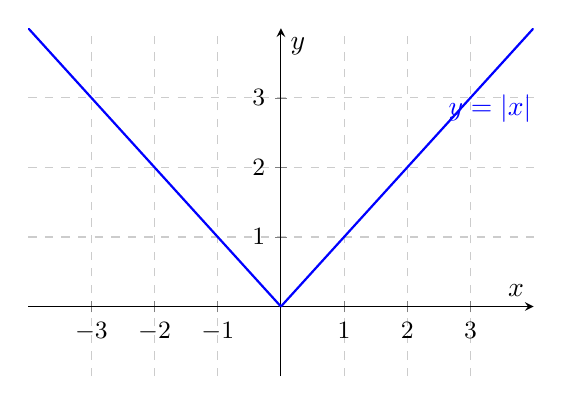
\begin{tikzpicture}
\begin{axis}[
    axis lines = center,
    xlabel = {$x$},
    ylabel = {$y$},
    xmin=-4, xmax=4,
    ymin=-1, ymax=4,
    xtick={-3,-2,-1,0,1,2,3},
    ytick={0,1,2,3},
    width=8cm, height=6cm,
    grid=major,
    grid style={dashed, gray!40},
    tick label style={font=\small},
]
\addplot[thick, blue, domain=-4:0, samples=50] {-x};
\addplot[thick, blue, domain=0:4, samples=50] {x};
\node[above right, blue] at (axis cs: 2.5, 2.5) {$y = |x|$};
\end{axis}
\end{tikzpicture}
\end{center}

\begin{remark}
Funkcijos $y = |x|$ savybės:
\begin{itemize}
    \item Apibrėžimo sritis: $D = \mathbb{R}$.
    \item Reikšmių sritis: $E = [0; +\infty)$.
    \item Funkcija \textbf{lyginė}: $|{-x}| = |x|$, t.~y.\ grafikas simetriška $Oy$ ašies atžvilgiu.
    \item Mažiausia reikšmė $y = 0$ pasiekiama taške $x = 0$.
\end{itemize}
\end{remark}

\subsubsection*{Transformacijos: \texorpdfstring{$y = |f(x)|$}{y = |f(x)|}}

Turint funkcijos $y = f(x)$ grafiką, funkcijos $y = |f(x)|$ grafikas gaunamas tokiu būdu:
\begin{itemize}
    \item ta grafiko dalis, kuri yra \textbf{virš} $Ox$ ašies (t.~y.\ $f(x) \geq 0$), \textbf{lieka nepakitusi};
    \item ta grafiko dalis, kuri yra \textbf{žemiau} $Ox$ ašies (t.~y.\ $f(x) < 0$), \textbf{atspindima} $Ox$ ašies atžvilgiu (t.~y.\ „apverčiama" aukštyn).
\end{itemize}

\begin{example}
Nubraižykite funkcijos $y = |x^2 - 4|$ grafiką.

\textbf{Sprendimas.}
Pirmiausia nubrėžiame $y = x^2 - 4$ – parabola su viršūne $(0, -4)$, kertanti $Ox$ ašį taškuose $x = -2$ ir $x = 2$. Tada:
\[
y = |x^2 - 4| = \begin{cases} x^2 - 4, & \text{jei } x \leq -2 \text{ arba } x \geq 2, \\ -(x^2 - 4) = 4 - x^2, & \text{jei } -2 < x < 2. \end{cases}
\]
Grafiko dalis, buvusi žemiau $Ox$ ašies (t.~y.\ intervale $(-2;\, 2)$), atspindima aukštyn.

\begin{center}
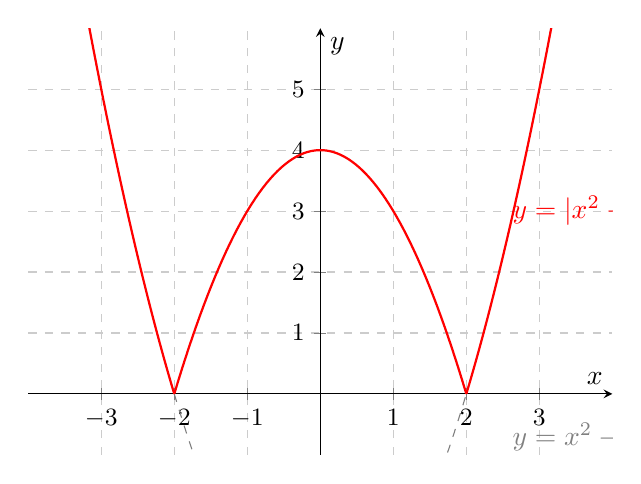
\begin{tikzpicture}
\begin{axis}[
    axis lines = center,
    xlabel = {$x$},
    ylabel = {$y$},
    xmin=-4, xmax=4,
    ymin=-1, ymax=6,
    xtick={-3,-2,-1,0,1,2,3},
    ytick={0,1,2,3,4,5},
    width=9cm, height=7cm,
    grid=major,
    grid style={dashed, gray!40},
    tick label style={font=\small},
]
% Original parabola (dashed, below x-axis part)
\addplot[dashed, gray, domain=-4:-2, samples=80] {x^2 - 4};
\addplot[dashed, gray, domain=2:4, samples=80] {x^2 - 4};
\addplot[dashed, gray, domain=-2:2, samples=80] {x^2 - 4};
% |f(x)| graph
\addplot[thick, red, domain=-4:-2, samples=80] {x^2 - 4};
\addplot[thick, red, domain=-2:2, samples=80] {4 - x^2};
\addplot[thick, red, domain=2:4, samples=80] {x^2 - 4};
\node[right, red] at (axis cs: 2.5, 3) {$y=|x^2-4|$};
\node[right, gray] at (axis cs: 2.5, -0.7) {$y=x^2-4$};
\end{axis}
\end{tikzpicture}
\end{center}
\end{example}

\subsubsection*{Transformacijos: \texorpdfstring{$y = f(|x|)$}{y = f(|x|)}}

Turint funkcijos $y = f(x)$ grafiką, funkcijos $y = f(|x|)$ grafikas gaunamas tokiu būdu:
\begin{itemize}
    \item ta grafiko dalis, kuri yra \textbf{dešinėje} $Oy$ ašies pusėje ($x \geq 0$), \textbf{lieka nepakitusi};
    \item ta grafiko dalis, kuri yra \textbf{kairėje} $Oy$ ašies pusėje ($x < 0$), \textbf{pašalinama};
    \item dešinės pusės grafikas \textbf{atspindimas} $Oy$ ašies atžvilgiu ir nukopijuojamas į kairę pusę.
\end{itemize}

\begin{remark}
Funkcija $y = f(|x|)$ visada yra \textbf{lyginė}: jos grafikas simetriška $Oy$ ašies atžvilgiu.
\end{remark}

\begin{example}
Nubraižykite funkcijos $y = f(|x|)$, kur $f(x) = x - 1$, grafiką.

\textbf{Sprendimas.}
\[
y = |x| - 1.
\]
Tai yra pagrindinės modulio funkcijos $y = |x|$ grafikas, pastumtas žemyn per 1 vienetą. Viršūnė – taške $(0, -1)$, grafiko šakos kerta $Ox$ ašį taškuose $x = -1$ ir $x = 1$.
\end{example}

\subsubsection*{Bendroji forma su parametrais}

Modulio funkcija su poslinkiais ir mastelio koeficientu:
\[
y = a\,|x - h| + k,
\]
kur:
\begin{itemize}
    \item $a$ – \textbf{mastelio koeficientas}: jei $|a| > 1$, grafiko šakos siauresnės (stačiau); jei $0 < |a| < 1$ – platesnės (švelniau). Jei $a < 0$, grafikas apverčiamas (viršūnė tampa aukščiausia, „$\Lambda$" forma).
    \item $h$ – \textbf{horizontalusis poslinkis}: grafiko viršūnė perstumta į $x = h$.
    \item $k$ – \textbf{vertikalusis poslinkis}: grafiko viršūnė perstumta į $y = k$.
    \item \textbf{Viršūnė} yra taške $(h,\, k)$.
\end{itemize}

\begin{center}
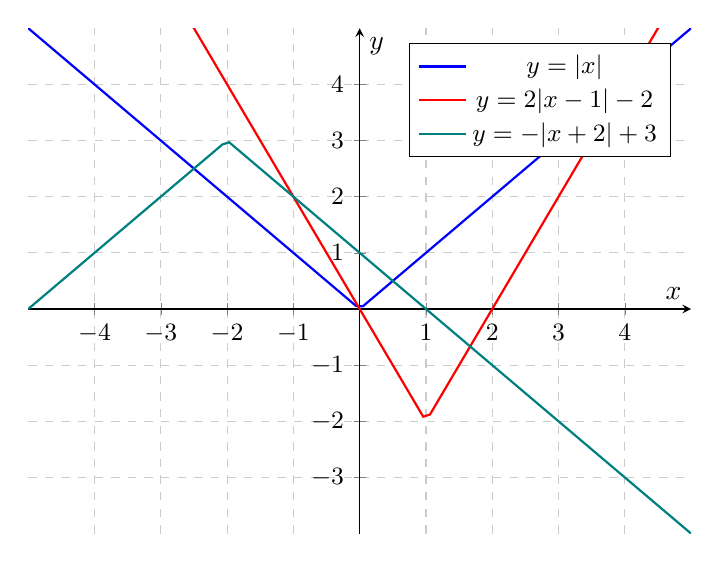
\begin{tikzpicture}
\begin{axis}[
    axis lines = center,
    xlabel = {$x$},
    ylabel = {$y$},
    xmin=-5, xmax=5,
    ymin=-4, ymax=5,
    xtick={-4,-3,-2,-1,0,1,2,3,4},
    ytick={-3,-2,-1,0,1,2,3,4},
    width=10cm, height=8cm,
    grid=major,
    grid style={dashed, gray!40},
    tick label style={font=\small},
    legend pos=north east,
    legend style={font=\small},
]
\addplot[thick, blue, domain=-5:5, samples=100] {abs(x)};
\addlegendentry{$y=|x|$}
\addplot[thick, red, domain=-5:5, samples=100] {2*abs(x-1)-2};
\addlegendentry{$y=2|x-1|-2$}
\addplot[thick, teal, domain=-5:5, samples=100] {-abs(x+2)+3};
\addlegendentry{$y=-|x+2|+3$}
\end{axis}
\end{tikzpicture}
\end{center}

\begin{example}
Nustatykite funkcijos $y = -2|x + 3| + 4$ grafiką: viršūnę, kryptį, šaknų koordinates.

\textbf{Sprendimas.}

\begin{itemize}
    \item Viršūnė: $h = -3$, $k = 4$, t.~y.\ taškas $(-3;\, 4)$.
    \item Kadangi $a = -2 < 0$, grafikas atviras \textbf{žemyn} ($\Lambda$ forma).
    \item Šaknys: $-2|x+3|+4 = 0 \Rightarrow |x+3| = 2 \Rightarrow x+3 = \pm 2$, taigi $x_1 = -1$, $x_2 = -5$.
\end{itemize}
\end{example}

% ─────────────────────────────────────────────────────────────────
\subsection{Sprendimas grafiškai}
% ─────────────────────────────────────────────────────────────────

Lygtys ir nelygybės su moduliais dažnai gali būti sprendžiamos \textbf{grafiškai} – nubrėžus abiejų pusių grafikus ir radus jų sankirtos taškus arba palyginus jų padėtis.

\subsubsection*{Lygčių sprendimas grafiškai}

\begin{definition}
Lygtis $f(x) = g(x)$ \textbf{grafinis sprendimas} – tai grafikų $y = f(x)$ ir $y = g(x)$ \textbf{sankirtos taškų abscisių} ($x$ koordinačių) radimas. Kiekviena sankirta atitinka vieną sprendinį.
\end{definition}

\textbf{Algoritmas:}
\begin{enumerate}
    \item Užrašykite lygtį pavidalu $f(x) = g(x)$.
    \item Toje pačioje koordinačių sistemoje nubraižykite abu grafikus.
    \item Raskite jų sankirtos taškus.
    \item Atskaitykite arba apskaičiuokite sankirtos taškų $x$ koordinates – tai ir yra sprendiniai.
\end{enumerate}

\begin{example}
Grafiškai išspręskite lygtį $|x - 1| = 2$.

\textbf{Sprendimas.}

Nubrėžiame $y = |x-1|$ (modulio funkcija, viršūnė $(1,0)$) ir tiesę $y = 2$. Jos susikerta dviejuose taškuose:

\[
|x-1| = 2 \implies x - 1 = 2 \;\text{ arba }\; x - 1 = -2 \implies x_1 = 3,\quad x_2 = -1.
\]

\begin{center}
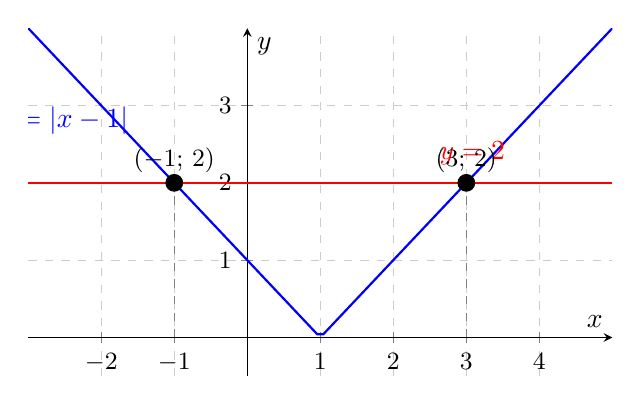
\begin{tikzpicture}
\begin{axis}[
    axis lines = center,
    xlabel = {$x$},
    ylabel = {$y$},
    xmin=-3, xmax=5,
    ymin=-0.5, ymax=4,
    xtick={-2,-1,0,1,2,3,4},
    ytick={0,1,2,3},
    width=9cm, height=6cm,
    grid=major,
    grid style={dashed, gray!40},
    tick label style={font=\small},
]
\addplot[thick, blue, domain=-3:5, samples=100] {abs(x-1)};
\node[above left, blue] at (axis cs: -1.5, 2.5) {$y=|x-1|$};
\addplot[thick, red, domain=-3:5] {2};
\node[above right, red] at (axis cs: 2.5, 2.1) {$y=2$};
% Intersection points
\addplot[only marks, mark=*, mark size=3pt, black] coordinates {(3,2) (-1,2)};
\node[above] at (axis cs: 3, 2) {\small $(3;\,2)$};
\node[above] at (axis cs: -1, 2) {\small $(-1;\,2)$};
% Dashed vertical lines
\addplot[dashed, gray] coordinates {(3,0)(3,2)};
\addplot[dashed, gray] coordinates {(-1,0)(-1,2)};
\end{axis}
\end{tikzpicture}
\end{center}

\textbf{Atsakymas:} $x_1 = -1$, $x_2 = 3$.
\end{example}

\begin{example}
Grafiškai išspręskite lygtį $|2x - 3| = x$.

\textbf{Sprendimas.}

Nubrėžiame $y = |2x-3|$ (viršūnė $\bigl(\tfrac{3}{2};\, 0\bigr)$, šakos nuolydžiai $\pm 2$) ir tiesę $y = x$.

\begin{center}
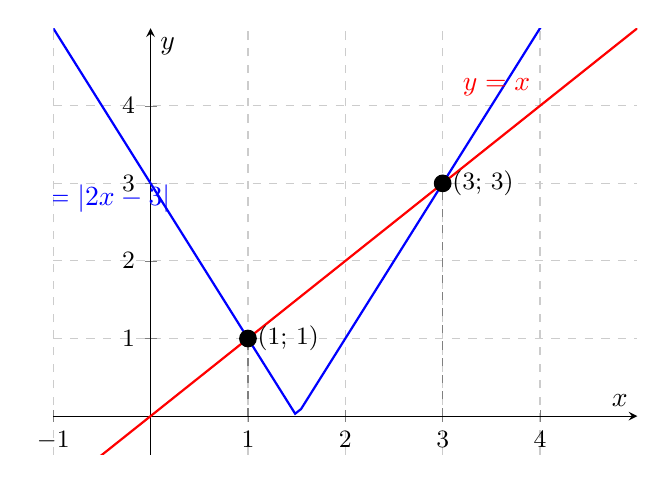
\begin{tikzpicture}
\begin{axis}[
    axis lines = center,
    xlabel = {$x$},
    ylabel = {$y$},
    xmin=-1, xmax=5,
    ymin=-0.5, ymax=5,
    xtick={-1,0,1,2,3,4},
    ytick={0,1,2,3,4},
    width=9cm, height=7cm,
    grid=major,
    grid style={dashed, gray!40},
    tick label style={font=\small},
]
\addplot[thick, blue, domain=-1:5, samples=100] {abs(2*x-3)};
\node[above left, blue] at (axis cs: 0.3, 2.5) {$y=|2x-3|$};
\addplot[thick, red, domain=-1:5] {x};
\node[above left, red] at (axis cs: 4, 4) {$y=x$};
% Intersections: x=1 and x=3
\addplot[only marks, mark=*, mark size=3pt, black] coordinates {(1,1)(3,3)};
\node[right] at (axis cs: 1, 1) {\small $(1;\,1)$};
\node[right] at (axis cs: 3, 3) {\small $(3;\,3)$};
\addplot[dashed, gray] coordinates {(1,0)(1,1)};
\addplot[dashed, gray] coordinates {(3,0)(3,3)};
\end{axis}
\end{tikzpicture}
\end{center}

Grafikai susikerta taškuose $x = 1$ ir $x = 3$. Tikriname algebriškai:
\begin{itemize}
    \item $x=1$: $|2\cdot1-3| = 1 = x$ \checkmark
    \item $x=3$: $|2\cdot3-3| = 3 = x$ \checkmark
\end{itemize}

\textbf{Atsakymas:} $x_1 = 1$, $x_2 = 3$.
\end{example}

\subsubsection*{Nelygybių sprendimas grafiškai}

\begin{definition}
Nelygybės $f(x) > g(x)$ \textbf{grafinis sprendimas} – tai $x$ reikšmių aibės radimas, kurioje grafikas $y = f(x)$ yra \textbf{aukščiau} grafiko $y = g(x)$. Analogiškai $f(x) < g(x)$ – tai sritis, kurioje $y = f(x)$ yra \textbf{žemiau} $y = g(x)$.
\end{definition}

\textbf{Algoritmas:}
\begin{enumerate}
    \item Nubrėžkite abu grafikus toje pačioje koordinačių sistemoje.
    \item Raskite sankirtos taškų abscises – tai \textbf{kritiniai taškai}.
    \item Nustatykite, kuriuose intervaluose vienas grafikas yra virš kito.
    \item Užrašykite sprendinių aibę intervalo pavidalu.
\end{enumerate}

\begin{example}
Grafiškai išspręskite nelygybę $|x + 2| \leq 3$.

\textbf{Sprendimas.}

Nubrėžiame $y = |x+2|$ (viršūnė $(-2;\,0)$) ir tiesę $y = 3$.

Grafikai susikerta, kai $x = 1$ (dešinė pusė: $x+2 = 3$) ir $x = -5$ (kairė pusė: $-(x+2) = 3$).

\begin{center}
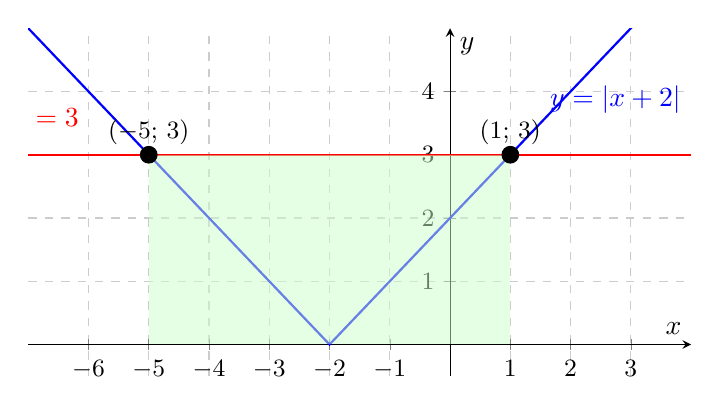
\begin{tikzpicture}
\begin{axis}[
    axis lines = center,
    xlabel = {$x$},
    ylabel = {$y$},
    xmin=-7, xmax=4,
    ymin=-0.5, ymax=5,
    xtick={-6,-5,-4,-3,-2,-1,0,1,2,3},
    ytick={0,1,2,3,4},
    width=10cm, height=6cm,
    grid=major,
    grid style={dashed, gray!40},
    tick label style={font=\small},
]
\addplot[thick, blue, domain=-7:4, samples=100] {abs(x+2)};
\node[above right, blue] at (axis cs: 1.5, 3.5) {$y=|x+2|$};
\addplot[thick, red, domain=-7:4] {3};
\node[above left, red] at (axis cs: -6, 3.2) {$y=3$};
% Solution region
\addplot[fill=green!20, opacity=0.5, draw=none] coordinates {(-5,0)(-5,3)(1,3)(1,0)};
\addplot[only marks, mark=*, mark size=3pt, black] coordinates {(-5,3)(1,3)};
\node[above] at (axis cs: -5, 3) {\small $(-5;\,3)$};
\node[above] at (axis cs: 1, 3) {\small $(1;\,3)$};
\end{axis}
\end{tikzpicture}
\end{center}

Modulio grafikas yra \textbf{žemiau arba ant} tiesės $y = 3$ intervale $[-5;\, 1]$.

\textbf{Atsakymas:} $x \in [-5;\, 1]$.
\end{example}

\begin{example}
Grafiškai išspręskite nelygybę $|x - 1| > x + 1$.

\textbf{Sprendimas.}

Nubrėžiame $y_1 = |x-1|$ ir $y_2 = x+1$. Sankirtos taškai:
\begin{itemize}
    \item Kai $x \geq 1$: $x - 1 = x + 1 \Rightarrow -1 = 1$ – prieštara, nėra sankirtos.
    \item Kai $x < 1$: $-(x-1) = x+1 \Rightarrow 1-x = x+1 \Rightarrow 0 = 2x \Rightarrow x = 0$.
\end{itemize}

Taigi grafikai susikerta tik taške $x = 0$, $y = 1$.

\begin{center}
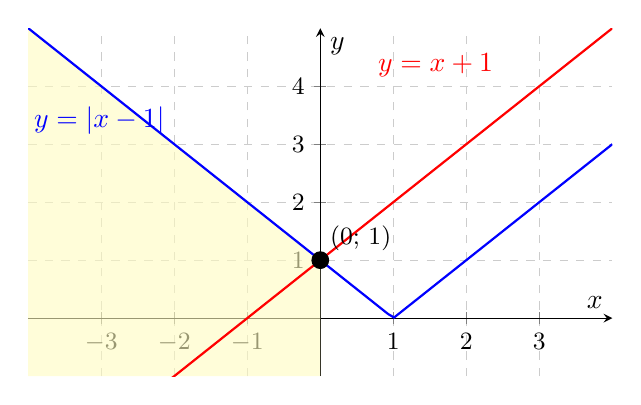
\begin{tikzpicture}
\begin{axis}[
    axis lines = center,
    xlabel = {$x$},
    ylabel = {$y$},
    xmin=-4, xmax=4,
    ymin=-1, ymax=5,
    xtick={-3,-2,-1,0,1,2,3},
    ytick={0,1,2,3,4},
    width=9cm, height=6cm,
    grid=major,
    grid style={dashed, gray!40},
    tick label style={font=\small},
]
\addplot[fill=yellow!25, opacity=0.6, draw=none] coordinates {(-4,5)(-4,-1)(0,-1)(0,1)};
\addplot[thick, blue, domain=-4:4, samples=100] {abs(x-1)};
\node[above left, blue] at (axis cs: -2, 3) {$y=|x-1|$};
\addplot[thick, red, domain=-4:4] {x+1};
\node[above left, red] at (axis cs: 2.5, 4) {$y=x+1$};
\addplot[only marks, mark=*, mark size=3pt, black] coordinates {(0,1)};
\node[above right] at (axis cs: 0, 1) {\small $(0;\,1)$};
\end{axis}
\end{tikzpicture}
\end{center}

Iš grafiko matyti, kad $y_1 > y_2$ (modulio grafikas aukščiau tiesės), kai $x < 0$.

\textbf{Atsakymas:} $x \in (-\infty;\, 0)$.
\end{example}

\subsubsection*{Sprendinių skaičiaus nustatymas grafiškai}

Grafinis metodas ypač naudingas, kai reikia \textbf{nustatyti sprendinių skaičių} neišsprendus lygties tiksliai. Pavyzdžiui, norint sužinoti, kiek sprendinių turi lygtis $|x^2 - 2| = k$ (kur $k$ – parametras), galima tyrinėti, kaip horizontali tiesė $y = k$ kerta grafiką $y = |x^2 - 2|$:

\begin{itemize}
    \item $k < 0$: \textbf{nėra sprendinių} (tiesė žemiau grafiko).
    \item $k = 0$: \textbf{du sprendiniai} ($x = \pm\sqrt{2}$).
    \item $0 < k < 2$: \textbf{keturi sprendiniai}.
    \item $k = 2$: \textbf{trys sprendiniai} ($x = 0$ ir $x = \pm 2$).
    \item $k > 2$: \textbf{du sprendiniai}.
\end{itemize}

\begin{center}
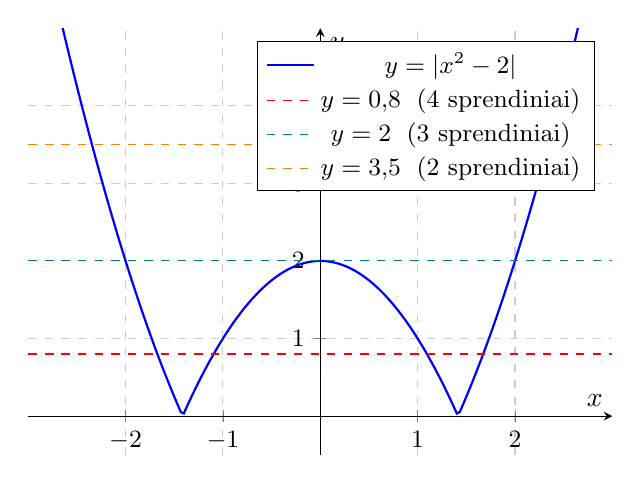
\begin{tikzpicture}
\begin{axis}[
    axis lines = center,
    xlabel = {$x$},
    ylabel = {$y$},
    xmin=-3, xmax=3,
    ymin=-0.5, ymax=5,
    xtick={-2,-1,0,1,2},
    ytick={0,1,2,3,4},
    width=9cm, height=7cm,
    grid=major,
    grid style={dashed, gray!40},
    tick label style={font=\small},
    legend pos=north east,
    legend style={font=\small},
]
\addplot[thick, blue, domain=-3:3, samples=200] {abs(x^2 - 2)};
\addlegendentry{$y=|x^2-2|$}
\addplot[dashed, red, domain=-3:3] {0.8};
\addlegendentry{$y=0{,}8$\; (4 sprendiniai)}
\addplot[dashed, teal, domain=-3:3] {2};
\addlegendentry{$y=2$\; (3 sprendiniai)}
\addplot[dashed, orange, domain=-3:3] {3.5};
\addlegendentry{$y=3{,}5$\; (2 sprendiniai)}
\end{axis}
\end{tikzpicture}
\end{center}

\begin{exercise}
Kiek sprendinių turi lygtis $|3x - 6| = k$, jei:
\begin{enumerate}[label=\alph*)]
    \item $k = -1$,
    \item $k = 0$,
    \item $k = 4$?
\end{enumerate}
\textit{Atsakymas:} a) nėra sprendinių; b) vienas sprendinys ($x=2$); c) du sprendiniai.
\end{exercise}

\begin{exercise}
Grafiškai išspręskite nelygybę $|2x + 1| \geq x + 2$ ir užrašykite sprendinių aibę.
\end{exercise}

\begin{exercise}
Nubrėžkite funkcijos $y = |x^2 - 3x + 2|$ grafiką ir nustatykite, su kuriomis $k$ reikšmėmis lygtis $|x^2 - 3x + 2| = k$ turi lygiai du sprendinius.
\end{exercise}

